%!TEX root = ../Systementwurf.tex

\chapter{Verteilungsentwurf}

Die wesentliche Funktionalität des \NewsGenie wird von den Hardware-Komponenten
\textit{Server} und \textit{Client} zur Verfügung gestellt. Desweiteren kann
über einen beliebigen Webbrowser auf das \textit{Webinterface} zur
Konfigurationen zugegriffen werden. Auf dem \textit{Web PC} muss also keine
spezielle Software installiert sein.

Die Kommunikation zwischen Server und Client erfolgt durch serialisierte
Java-Objekte mithilfe des Akka-Frameworks über das TCP/IP Protokoll. Das
Webinterface kommuniziert über HTTP(S).

\begin{figure}[h]
\centering
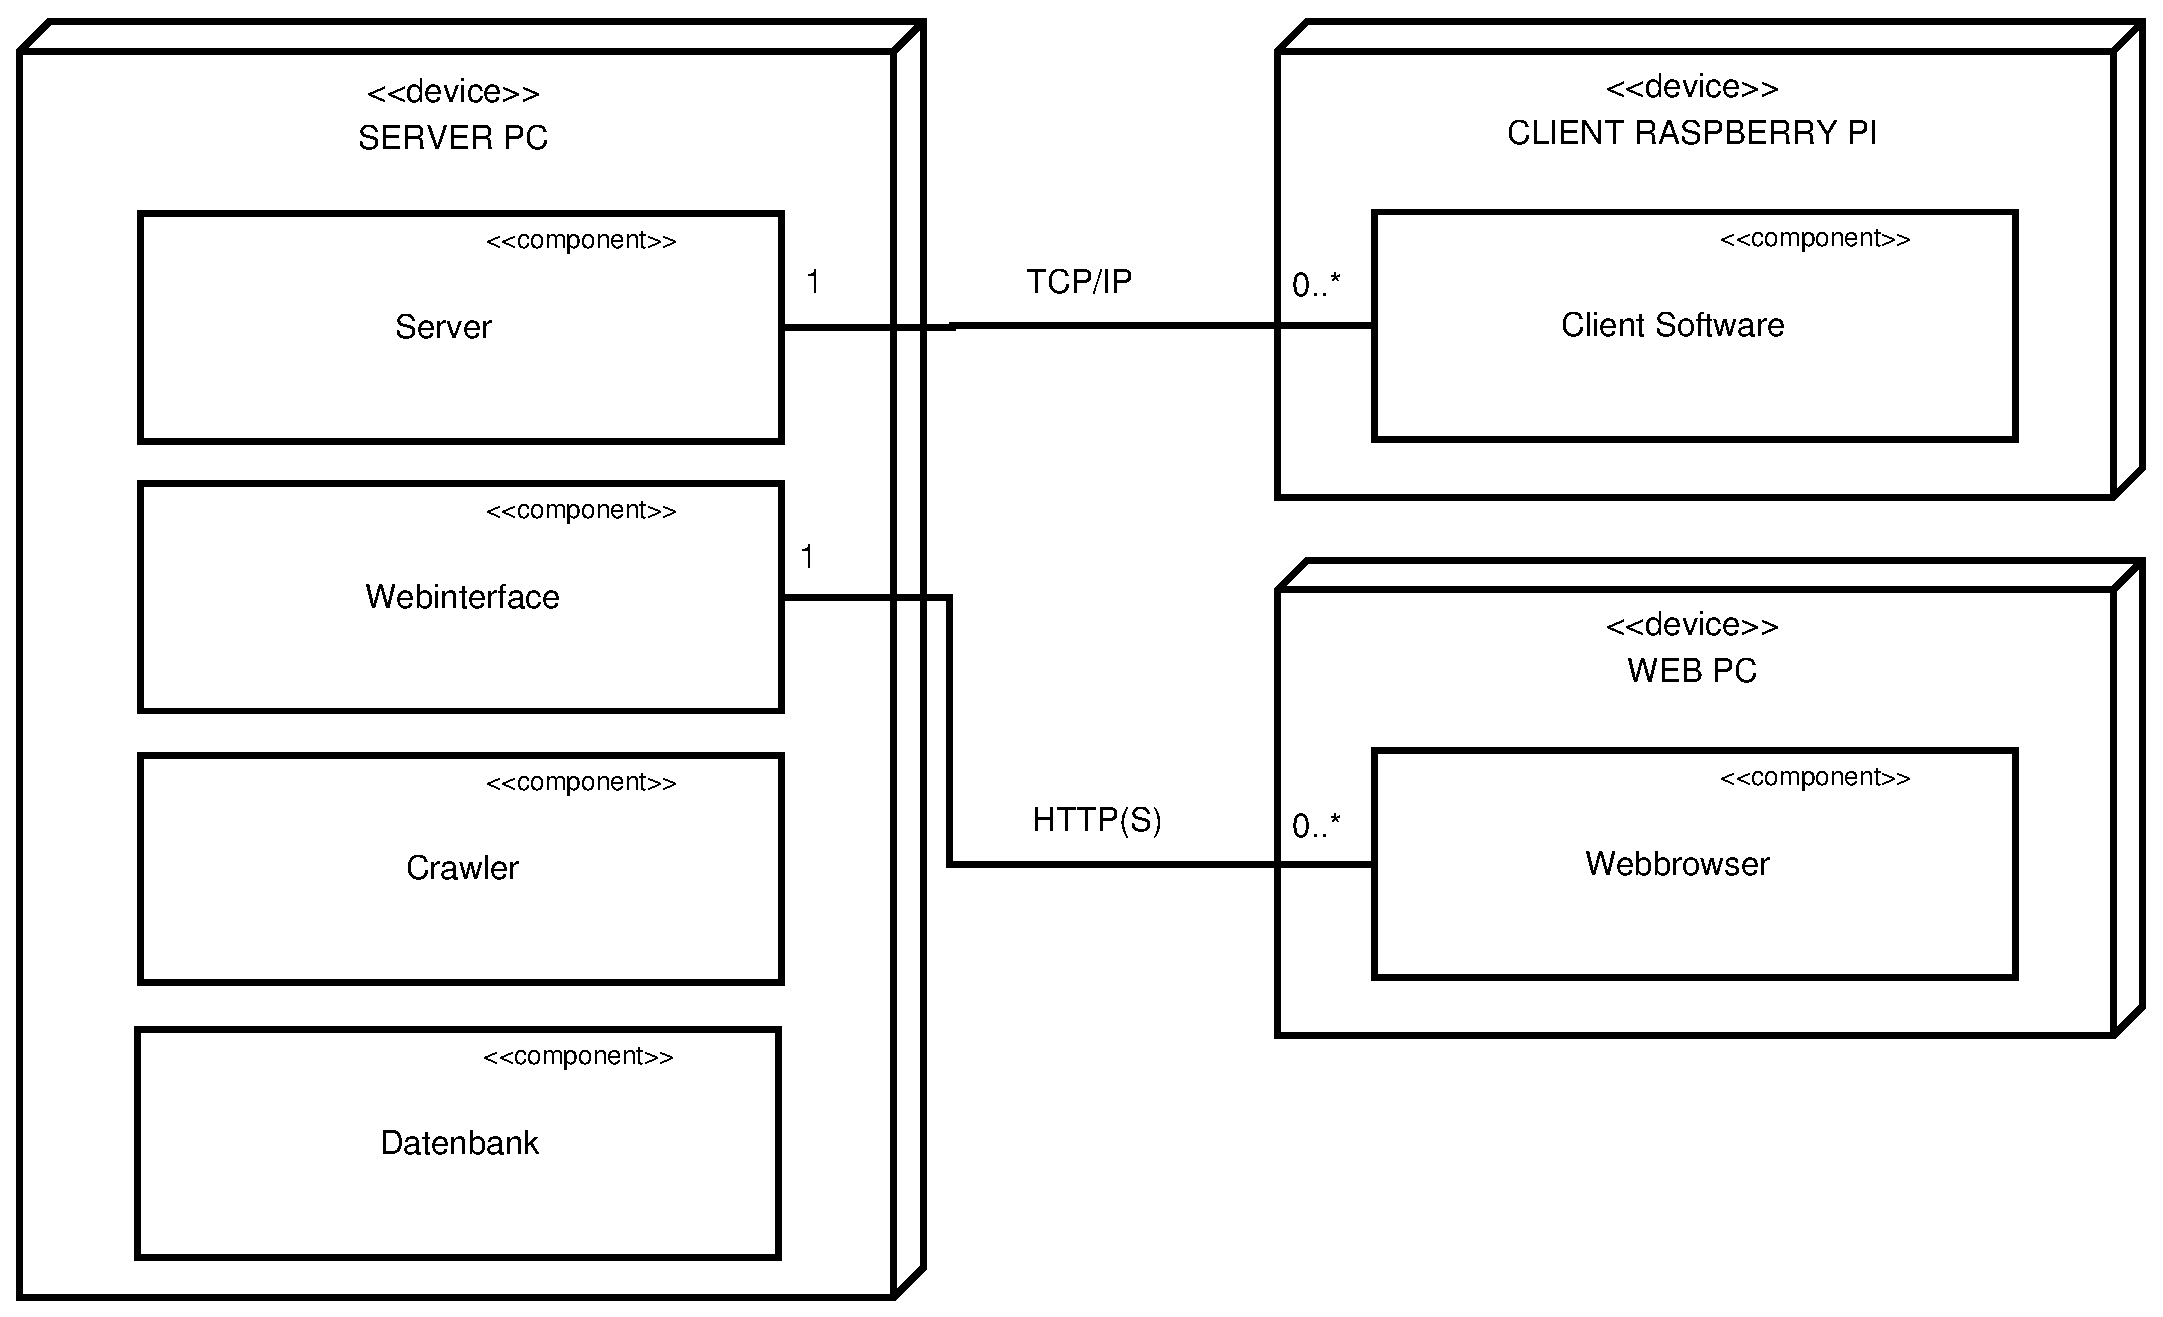
\includegraphics[width=1\textwidth]{Systementwurf/04_verteilungsentwurf/verteilungsentwurf.eps}
\caption{Verteilungsdiagramm}
\end{figure}